\documentclass{ifacconf}

\usepackage{amsmath}
\usepackage{amssymb}
\usepackage{multirow}
\usepackage{xcolor}
\usepackage{booktabs} 
\usepackage{setspace} 
\usepackage{tablefootnote}
\usepackage{float}

\usepackage{graphicx}      % include this line if your document contains figures
\usepackage{natbib}        % required for bibliography
% \bibliographystyle{IEEEtranS}
% \bibliographystyle{ifacconf}

\graphicspath{{../figures}}

%===============================================================================
\begin{document}
\setstretch{1.0}

\begin{frontmatter}

\title{Projecting presence of heart disease from clinical measures with statistical models}
% Title, preferably not more than 10 words.

\author{Nguyen Hoang The Kiet} 

\address{Bachelor Student in Data Science and Analytics, College of Humanities and Science, National University of Singapore (Email: e1375598@u.nus.edu).}

% \begin{abstract}                % Abstract of not more than 250 words.
% This article proposes to obtain a statistical model of the daily peak electricity load  of a household located in Austin-TX,USA. The Box-Jenkins methodology was followed to obtain the best fit for the time-series. Four models provided a good fit: ARIMA(0,1,2),  ARIMA(1,1,2), SARIMA(0,1,2)(0,1,1) and SARIMA(1,1,2)(0,1,1). The model with the highest Akaike Information Criteria was the ARIMA(1,2,2). However, the model with the highest forecast accuracy was the SARIMA(1,1,2)(0,1,1), which obtained an RMSE of 0.296 and a MAPE Of 15.00.

% \end{abstract}

\begin{keyword}
Statistical Modeling, Feature Extraction, \( k \)-NN, Decision Tree, Logistic Regression
\end{keyword}

\end{frontmatter}
%===============================================================================

\section{Introduction}

% This article proposes to obtain a statistical model of the daily peak electricity load  of a household located in Austin-TX,USA. The data was gathered from the Pecan Street Project Database of the University of Texas at Austin. They account for minute-to-minute electricity use during the year of 2015 of the house (a total of 525600 observations)
% The programming language Python was used to create an algorithm to find the maximum minute-load of a day, for all the 365 days of the year. This data then served as input for for the statistical modeling, which was performed in the programming language R. 
% The data was separated between training data (first 10 months and test data (last two months). The training data was used to identify the model and the test data for the accuracy of the forecast. The next section will explain the methodology and then apply it to the case study. 

This report proposes a statistical model to predict whether a patient has symptoms of heart disease. The cleaned data was given prior to the analysis, which contains a mixture of categorical and numerical features determining the patient's demographics and clinical measures. Experiments are conducted on three different types of models: $k$-Nearest Neighbours ($k$-NN), Decision Trees and Logistic Regression. Models are evaluated based on sensitivity (true positive rate, or TPR) with \( 5 \)-fold validation, from which the best model from each of its kind is selected and compared based on ROC-AUC \textit{(Receiver Operating Characteristic - Area Under the Curve)} and Precision-Recall tradeoffs.
\begin{table}[h]
    \centering
    \begin{tabular}{lllr}
    \toprule
    \textbf{feature} 
        & \textbf{type}
        & \textbf{description}
        & \textbf{NA}
        \\
    \midrule
    sex 
        & \texttt{fct(2)}
        & demographical
        & 0
        \\ 
    \midrule
    chest.pain 
        & \texttt{fct(4)}
        & clinical
        & 0
        \\
    \midrule
    fbs 
        & \texttt{fct(2)}
        & clinical
        & 0
        \\
    \midrule
    rest.ecg 
        & \texttt{fct(3)}
        & clinical
        & 0
        \\
    \midrule
    angina 
        & \texttt{fct(2)}
        & clinical
        & 0
        \\
    \midrule
    blood.disorder 
        & \texttt{fct(3)}
        & clinical
        & {\color{red} 2}
        \\
    \midrule
    age 
        & \texttt{int}
        & demographical
        & 0
        \\
    \midrule
    bp 
        & \texttt{int}
        & clinical
        & 0
        \\
    \midrule
    chol 
        & \texttt{int}
        & clinical
        & 0
        \\
    \midrule
    heart.rate 
        & \texttt{int}
        & clinical
        & 0
        \\
    \midrule
    vessels 
        % & \texttt{\color{red} int/fct(4)}
        & \texttt{int}
        & clinical
        & 0

        \\
    \midrule
    st.depression 
        & \texttt{dbl}
        & clinical
        & 0
        \\
    \bottomrule
    \toprule
    \textbf{response} 
        & \textbf{type}
        & \textbf{value}
        & \textbf{count}
        \\
    \midrule
    \multirow{2}{*}{disease}
        & \multirow{2}{*}{\texttt{fct(2)}}
        & 0 (absence) & 138*
        \\
        && 1 (presence) & 162*
        \\
    \bottomrule
\end{tabular}
    
    \raggedleft {\tiny (*) before NA exclusion}
    
    \vspace{4pt}
    \caption{Dataset features}
\end{table}

\section{Exploratory Data Analysis}


\subsection{Description of dataset}
The dataset comprises of \( 300 \) raw records and \( 12 \) different features. Although the data is already cleaned, there are 2 records with \( \texttt{blood.disorder} = 0 \), noting that no data was recorded in this field. We will simply remove these \( 2 \) records from our dataset.

\begin{table}[H]
    \centering
    \begin{tabular}{rrrrrr}
        \hline
        \textbf{Value} & 0 & 1 & 2 & 3 & Total\\
        \hline
        \textbf{Frequency} & 2 & 18 & 163 & 117 & \(n = 300\)\\
        \hline
    \end{tabular}
    \vspace{4pt}
    \caption{Frequency table of \texttt{blood.disorder}}
\end{table}


% \textbf{The \texttt{vessels} variable}. Despite being an integral feature, it only ranges from 0 to 4. For our purposes, we will consider \texttt{vessels} as a categorical variable of 5 factors \( \{0, 1, 2, 3, 4\} \).




\subsection{Categorical variables}
There are 6 categorical variables in the dataset, 5 of which are different types of clinical metrics 
(\texttt{angina}, \texttt{blood.disorder}, \texttt{chest.pain}, \texttt{fbs}, \texttt{rest.ecg}). In general, there is a disproportionate ratio of categories within the dataset. For example,
\begin{itemize}
    \item There are \textit{twice} the number of patients who experienced angina induced by exercise (\texttt{angina = 0}) compared to those that did not (\texttt{angina = 1});
    \item The number of patients having high fasting blood sugar level (\texttt{fbs = 1}) is about \textit{five times lower} than those having low fasting blood sugar level (\texttt{fbs = 0}).
\end{itemize}

\begin{figure}[h]
    \centering
    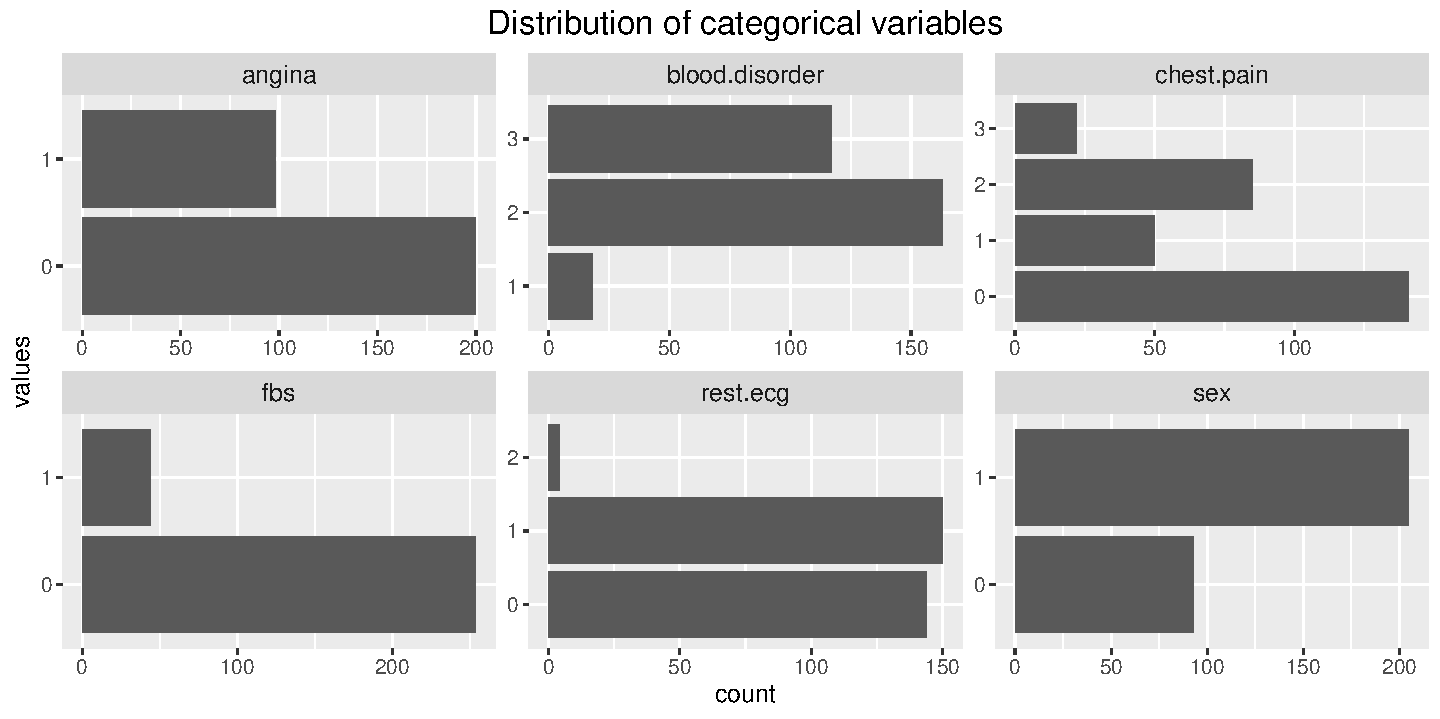
\includegraphics[width=\linewidth]{22.categorical.distribution.pdf}
    \caption{\centering Distribution of categorical variables}
\end{figure}

To test the significance of these features in predicting the presence of disease, two methods are used: \textit{percent stacked bar chart} and \textit{Fisher's exact test}. For a graphical inference, conditional probabilities \( \mathbb P[Y = y | X_i = x_i] \) (\( X_i \) being a categorical feature) are calculated and plotted on a \textit{percent stacked bar chart}. By visual inspection, it can be seen that the level of fasting blood sugar (\texttt{fbs}) is weakly correlated to the presence of disease. 

\begin{figure}[h]
    \centering
    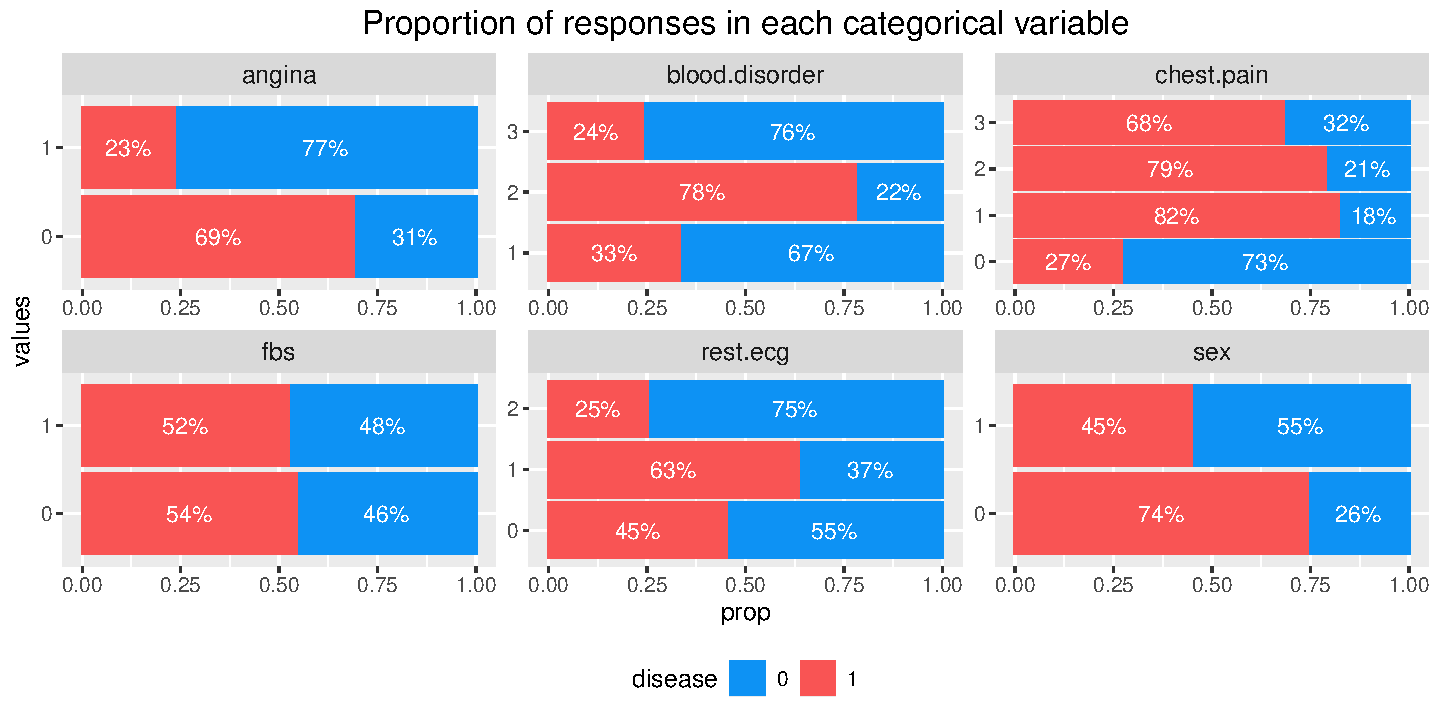
\includegraphics[width=\linewidth]{22.categorical.correlation.to.response.pdf}
    \caption{\centering Relationship of categorical features to the response variable}
\end{figure}

Indeed, one can calculate the odds ratio as
\begin{align*}
    \mathrm{OR} 
    &= 
    \frac{\mathbb P[Y = 1 | X = 1]}{\mathbb P[Y = 1 | X = 0]}\cdot
    \frac{\mathbb P[Y = 0 | X = 0]}{\mathbb P[Y = 0 | X = 1]}
    \\
    &\approx
    \frac{52\% \cdot 46\%}{54\% \cdot 48\%}
    \approx
    0.92
\end{align*}
which may suggests an insignificant correlation between fasting blood sugar and the presence of disease.

For a quantitative contigency test, \textit{Fisher's exact test} \citep{fishertest} is used. From applying Fisher's test, it is observed that there are
\begin{itemize}
    \item \textbf{No evidence of correlation} between the presence of disease and the categorical level of fasting blood sugar ($p > 10^{-2}$).
    \item \textbf{Correlation} between the presence of disease and other clinical measures ($p < 10^{-4}$).
\end{itemize}

\begin{table}[h]
    \centering
    \begin{tabular}{lr}
        \toprule
        \textbf{Variable} & \textbf{Fisher's p-value}\\
        \midrule
        angina          & $<$ 0.0001\\
        \midrule
        blood.disorder  & $<$ 0.0001\\
        \midrule
        chest.pain      & $<$ 0.0001\\
        \midrule
        \color{red}{fbs}        & \color{red}{0.8703}\\
        \midrule
        \color{gray}{rest.ecg}  & 0.0019\\
        \midrule
        sex             & $<$ 0.0001\\
        \bottomrule
    \end{tabular}
    
    \vspace{4pt}
    \caption{\centering Fisher's $p$-value for categorical variables}
\end{table}


\subsection{Numerical variables}
\begin{figure}[h]
    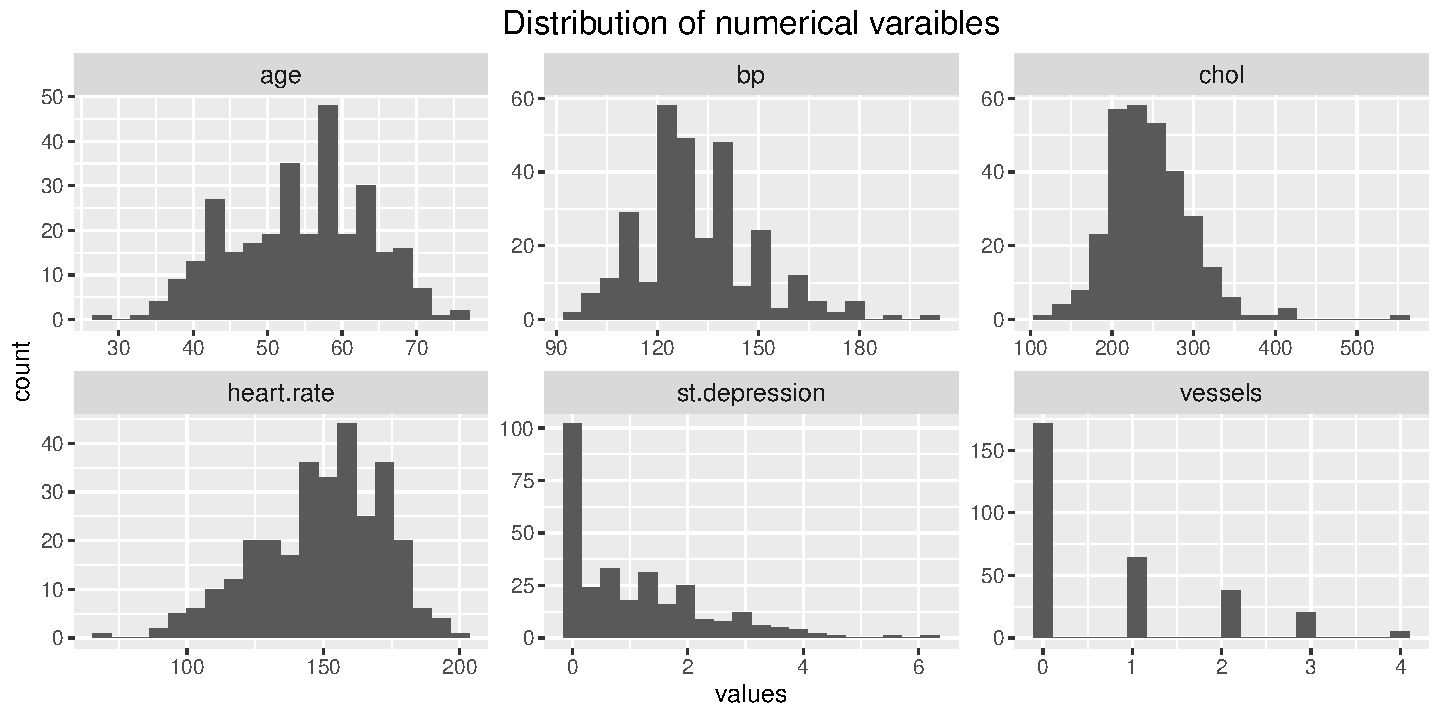
\includegraphics[width=\linewidth]{23.numerical.distribution.pdf}
    \caption{\centering Histogram of numerical features}
\end{figure}

There are 6 numerical variables in the dataset, 5 of which are different types of clinical metrics 
(\texttt{bp}, \texttt{chol}, \texttt{heart.rate}, \texttt{st.depression}, \texttt{vessels}). In general, by plotting the histograms for the variables, it is observed that some of the features (\texttt{bp}, \texttt{heart.rate}, \texttt{chol}) are 'close' to a normal distribution, whilst others are heavily \textit{left-skewed} (\texttt{age}) or \textit{right-skewed} (\texttt{st.depression}, \texttt{vessels}).


The relationship of number variables and the response is tested on a faceted box-plot. By visually comparing the distribution mean of each group, it can be seen that there are 

\begin{itemize}
    \item \textbf{Strong correlation} between varibles \texttt{age}, \texttt{heart.rate}, \texttt{vessels}, \texttt{st.depression} and the response variable;
    \item \textbf{Weak correlation} between \texttt{bp} and \texttt{chol} and the response variable
\end{itemize}

\begin{figure}[h]
    \centering
    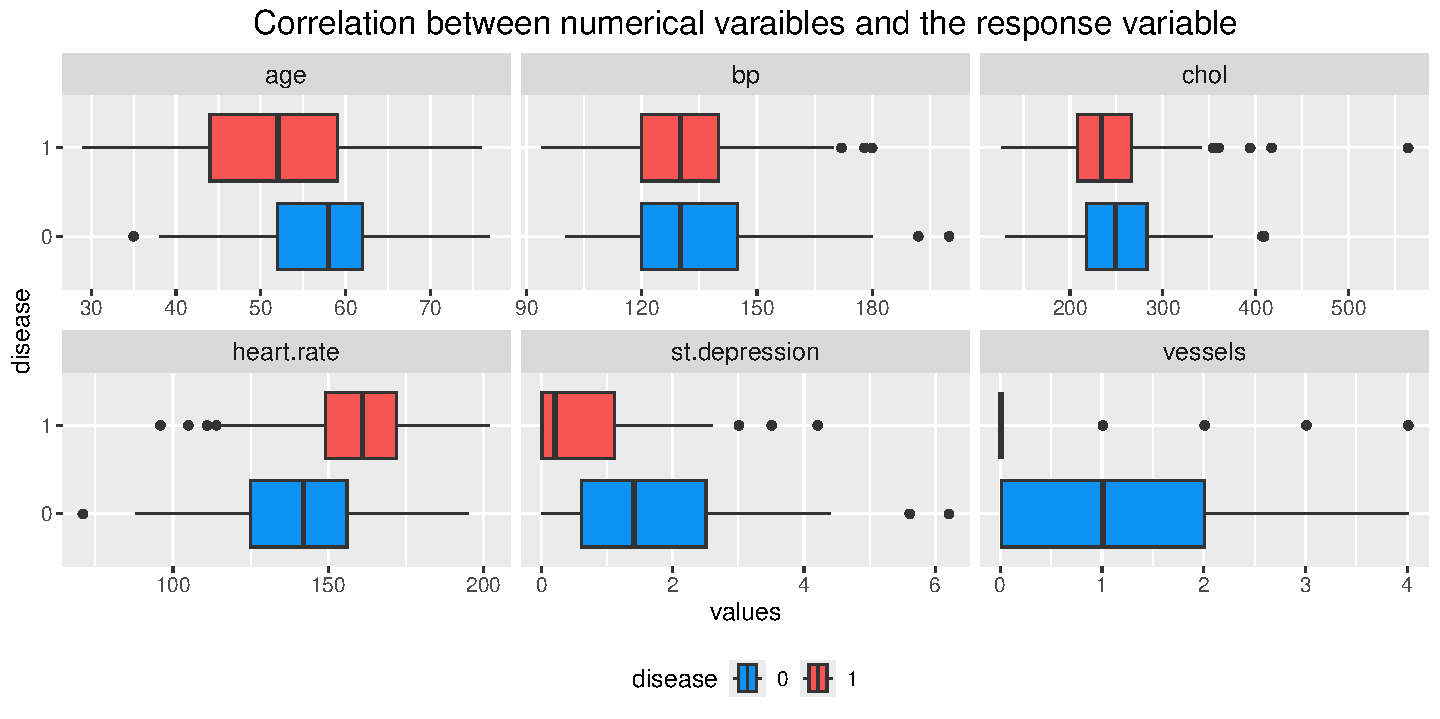
\includegraphics[width=\linewidth]{23.numerical.correlation.to.response.pdf}
    \caption{\centering Boxplot correlation with disease}
\end{figure}

To test for normality for each variables, a QQ-plot is used for visualisation, along with the p-value from the \textit{Shapiro-Wilk normality test} \citep{shapirotest}. As no variables are normally distributed (all \( p < 10^{-2} \)), normality transformations are also considered. In this case, the transformation of interest is the \textit{Box-Cox transformation}, a parametric transformation that generalises power and logarithmic transformations on positive variables with a single parameter \( \lambda \):

\[
    B_\lambda(x) = \begin{cases}
        \frac{x^\lambda - 1}{\lambda}   & \text{if \( \lambda \ne 0 \)} \\
        \ln{x}                          & \text{if \( \lambda  =  0 \)}
    \end{cases}
\]

For non-negative variables, a \( x \mapsto x + \varepsilon \) transformation, where \( \varepsilon = 0.01\), is applied before Box-Cox to prevent the transformation being undefined at \( x = 0 \).

Different values of \( \lambda \) in the range \( [-5, 5] \) are tested, the value of which yields the best \textit{Shapiro-Wilk's p-value} is retained. It can be observed that \texttt{age}, \texttt{bp}, \texttt{chol} and \texttt{heart.rate} are Box-Cox transformable to a normally distributed variable, within a \( 99\% \) level of significance. In contrast, heavy right-skewed variables (\texttt{st.depression} and \texttt{vessels}) fail to be normally transformable by the Box-Cox transformation.

\begin{figure}[h]
    \centering
    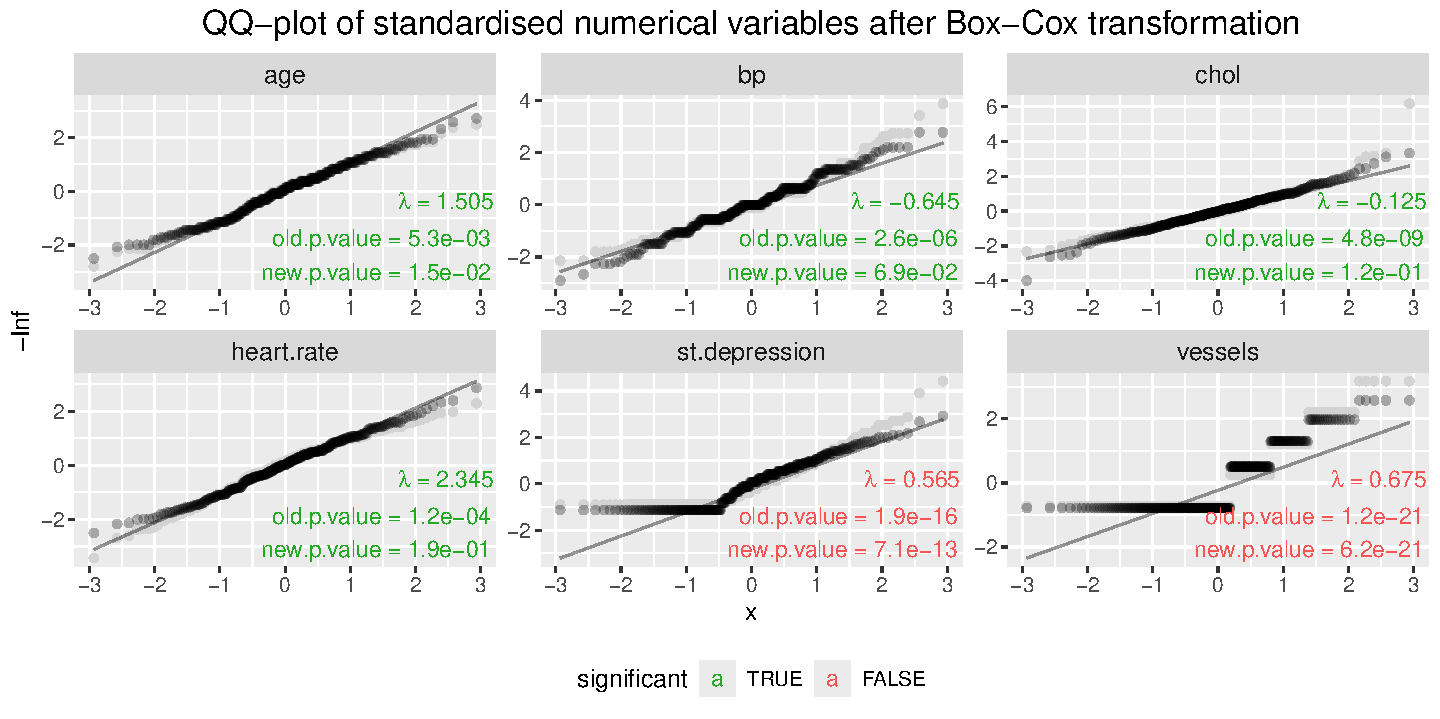
\includegraphics[width=\linewidth]{23.numerical.boxcox.qq.pdf}
    \caption{\centering Best Box-Cox transformation for each numerical variable}
\end{figure}



\subsection{Conclusion}
The dataset is a cleaned, 300-record dataset that shows the relationship between demographical and clinical features and the presence of heart disease. A combination of numerical and categorical variables are featured in this dataset, and whilst most features have strong correlation with the response variable, some features seem to be a weak predictor to heart disease (such as \texttt{fbs}, \texttt{bp} or \texttt{chol}). In further sections, models with or without this set of features will be tested against each other.
\section{Model Selection}

This report proposes the use of three families of models, \textit{\( k \)-Nearest neighbours, Decision trees and Logistic Regression}, in predicting the presence of disease through clinical measures. For each family of model, a range of hyperparameters are validated via \( 5 \)-fold cross-validation to choose the best candidate. Sensitivity (or True positive rate / TPR) is used as a reference to select the best performing model, with a caution that a high TPR needs not translate to good performance but rather due to underfitting, as the `True' label would be predicted at a impractical high probability.

To ease the fine-tuning process, a default of threshold of \( \delta = 0.5 \) is maintained throughout all models.

\subsection{\( k \)-Nearest neighbours (\( k \)-NN)}

\subsubsection{Methodology.}

\( k \)-Nearest neighbours (\( k \)-NN) is a simple, distance-based machine learning classification algorithm that lazily learns its class based on the majority class (for classification) or average value (for regression) of its nearest peers.

Due to \( k \)-NN's 'distance-based' nature, categorical features cannot be directly interpreted, hence they need to be transformed to numerical vectors. As in the dataset, most of the variables are numerical or ordinal values, the data is fed into the algorithm \textit{per se}, i.e., by \textit{label encoding}.

Another factor to be concerned of is feature scaling, as different measurements are made in different scales. Two scaling methods are tested: \textit{Normalisation}, where each feature is mapped to the range \( [0, 1] \) via a min-max transformation:

\begin{align*}
    \mathbf{x} \mapsto \frac{\mathbf x - \min\mathbf x}{\max\mathbf x - \min\mathbf x}
\end{align*}

and \textit{Box-Cox + Standardisation}, where each feature is fed to a Box-Cox transformation with its according optimal parameter \( \lambda \) (if applicable), then standardised:

\begin{align*}
    \mathbf{x} 
        \mapsto \mathbf{x'} := \frac{\mathbf{x}^\lambda - 1}\lambda  
        \mapsto \frac{\mathbf x' - \overline{\mathbf x'}}{\mathrm{std\ }\mathbf x'}
\end{align*}

\subsubsection{Experiments \& Results.}

\begin{table}[h]
    \centering
    \begin{tabular}{ccc}
        \toprule
        TPR, \( 19 \)-NN
        & \textbf{Full}
        & \textbf{Simplified\footnotemark{}}
        \\
        \midrule
        \textbf{Normalisation}
        & \( 86.274\% \)    
        & \( 88.697\% \)
        \\
        \midrule
        \textbf{Box-Cox + Standardisation}
        & \( 90.184\% \)    
        & \( 93.188\% \)
        \\
        \bottomrule
    \end{tabular}
    
    \raggedright
    \( ^1 \) {\small \texttt{fbs}, \texttt{bp} and \texttt{chol} are excluded from the model}
    
    \centering
    \vspace{4pt}
    \caption{\centering TPR performance of \( k \)-NN models, where \( k = 19 \)}
\end{table}

A total of four models are tested on a various range of values for \( k \in [3, 50]\), with a label cutoff at \( \delta = 0.5 \). It is observed that the simplified model with Box-Cox transformation followed by standardisation performed the best, with \( \text{TPR} = 93.94\% \) saturated at \( k \ge 19 \). 

\begin{figure}[H]
    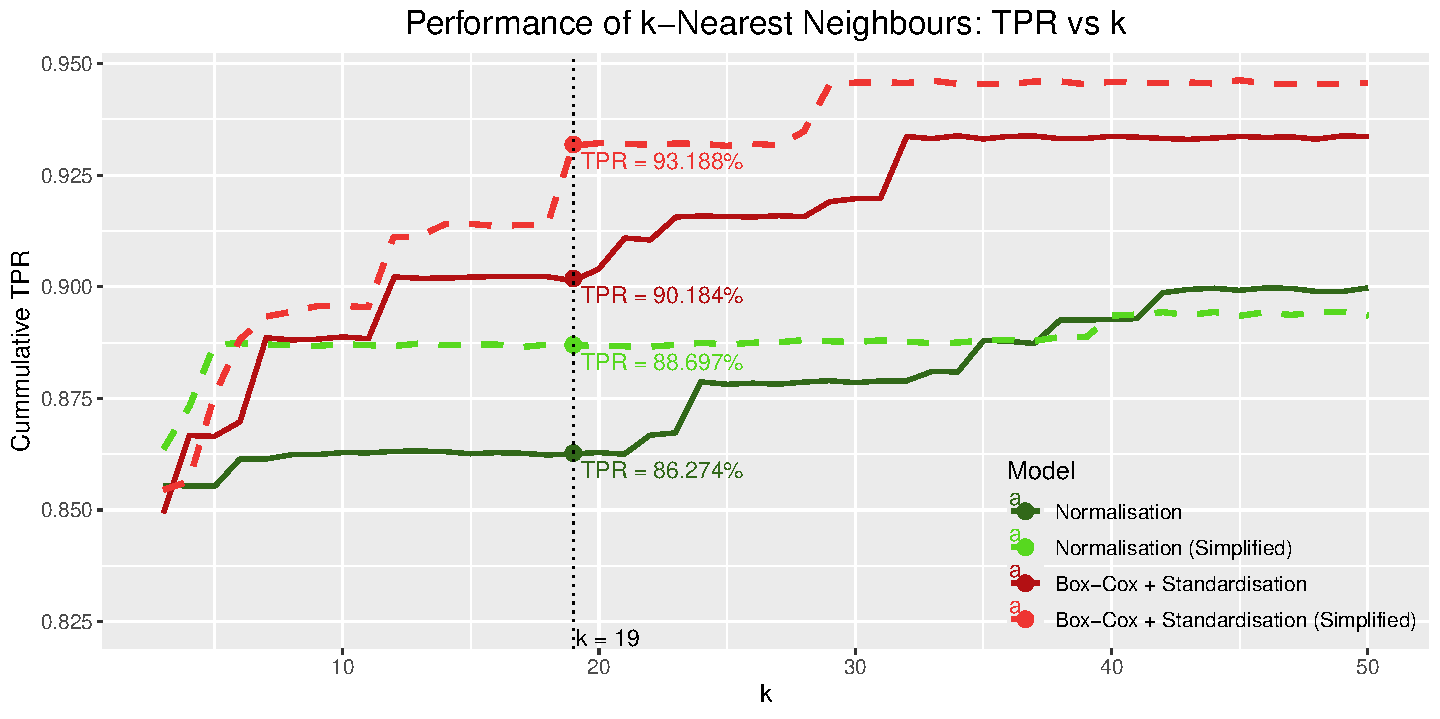
\includegraphics[width=\linewidth]{31.kNN.pdf}
    \caption{\centering TPR performance of \( k \)-NN models with running \(k\)}
\end{figure}
    
Generally, standardisation methods outperform normalsation as the best preprocessing method for \( k \)-NN. In terms of model complexity, simple models fit best for small values of \( k \), however when \( k \) gets larger, then simple models fit the data worse compared to full models; this may rather shows the effect of underfitting than outperformance. By the elbow method, it can be seen that the best performing model is a \textbf{\( 19 \)-nearest neighbour model on a Box-Cox, standardised dataset}.

\subsection{Decision tree}
\subsubsection{Methodology.}
Decision Tree is a rule-based machine learning algorithm, where its set of rules is generated by recursively splitting the dataset on a chosen feature so that the separation maximises a certain target criterion (e.g. entropy gain, Gini impurity, etc.). Despite being generally less accurate comparing to other machine learning models, it rises in terms of comprehensibility and explainability. As the algorithm does not assume the underlying distribution of the data, transformation such as standardisation or Box-Cox are not required at this stage.

\subsubsection{Experiments \& Results.}
Experiments focus in finding the best splitting algorithm, that includes the criterion to be optimised for splitting and the terminating condition. In other words, the following parameters are tested:

\begin{itemize}
    \item \textbf{\texttt{minsplit}}. Number of elements in a leaf node, where the algorithm stops splitting. \texttt{minsplit} is let to be \( 5, 10, 15, \cdots, 100 \);
    \item \textbf{\texttt{split}}. Algorithm to determine the optimal split. Either 'Information gain' (Entropy gain) or 'Gini impurity'.
\end{itemize}

In terms of sensitivity at \( \delta = 0.5 \), entropy-based algorithms fit well for a low \texttt{minsplit}, but as \texttt{minsplit} increases, its performance stagnated, both in the full or simplified tree. In contrast, Gini-based trees underperform with low values of \texttt{minsplit}, but gradually improve when \texttt{minsplit} increases. There is also an observation that simplifing the input does not change the metrics for large \texttt{minsplit}s, suggesting the possibility that the algorithm abandons these uncorrelated features at its internal procedures.

\begin{figure}[h]
    \centering
    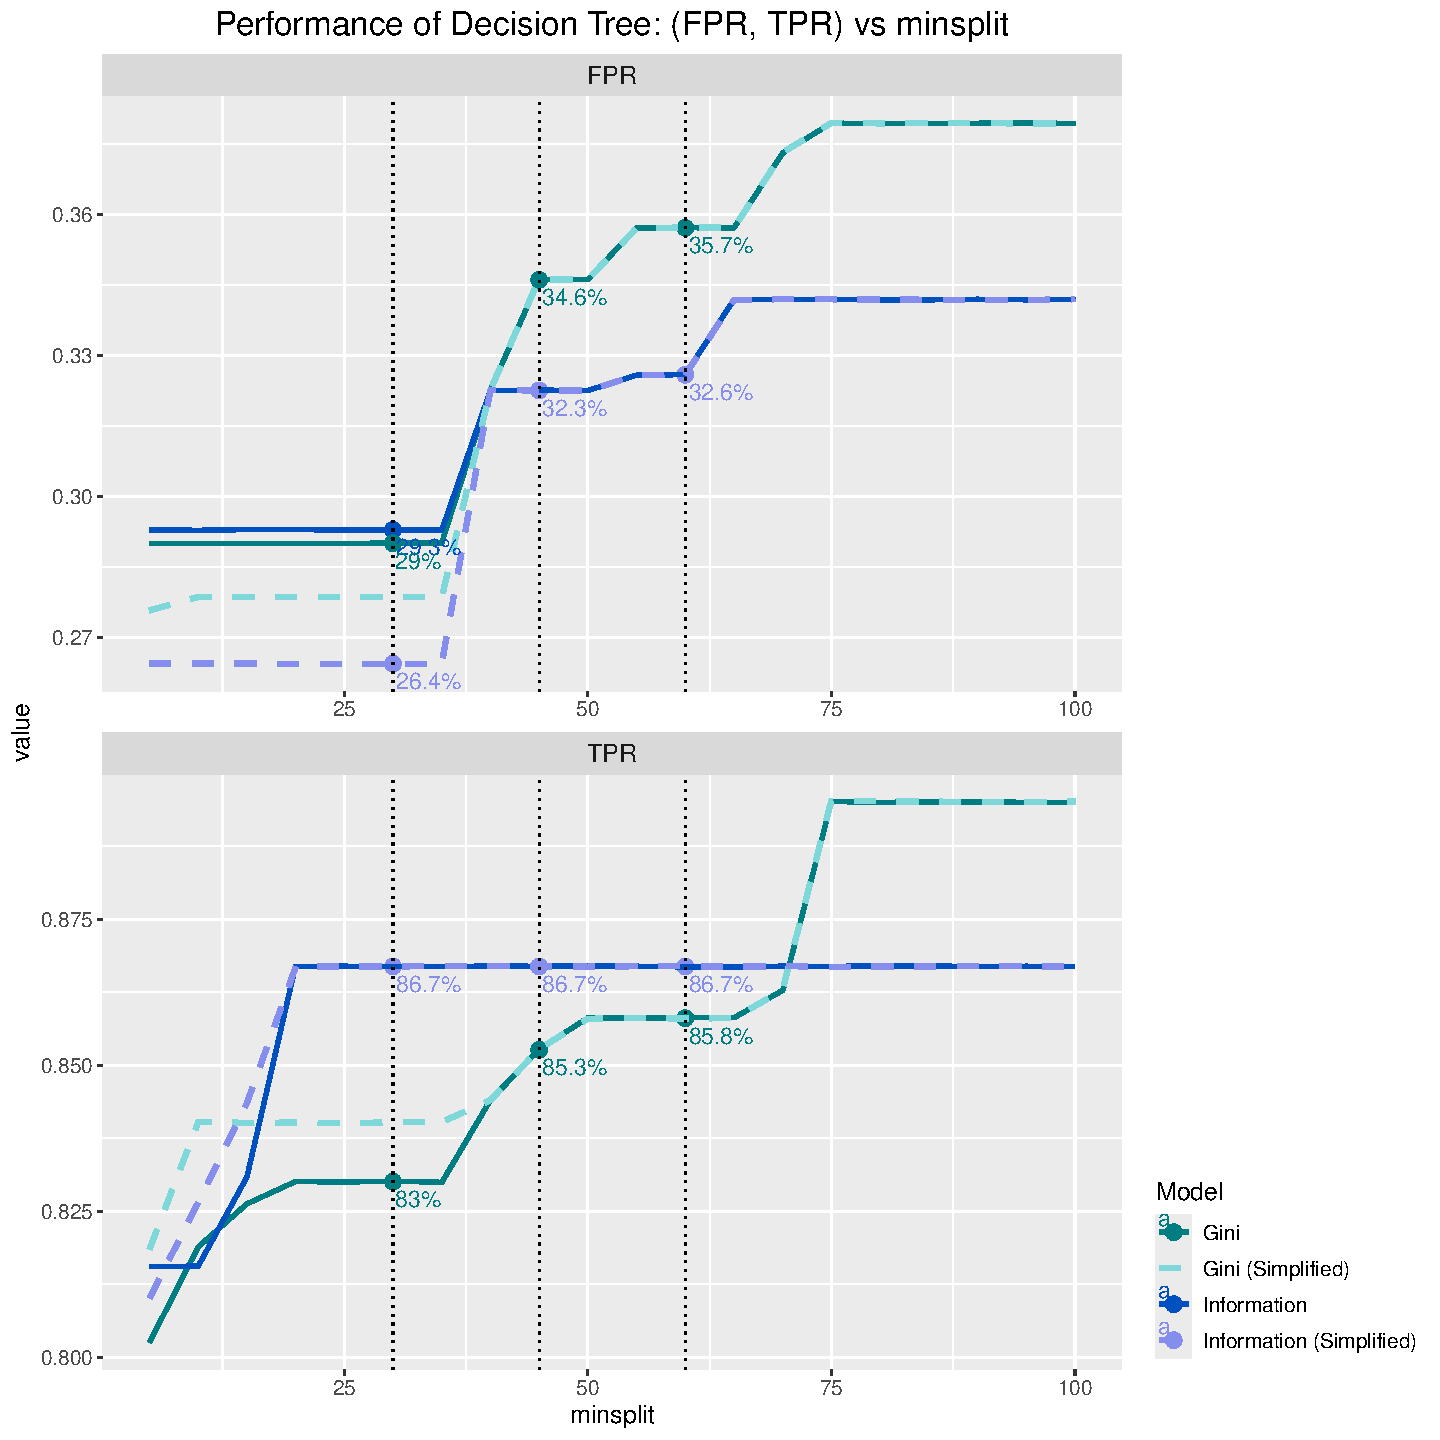
\includegraphics[width=\linewidth]{32.DecisionTree.pdf}
    \caption{\centering TPR/FPR performance of decision trees vs. minsplit}
\end{figure}

One should be cautious, however, when setting a high value of \texttt{minsplit}, as it would result in an underfitting tree with most of the datapoint classified as True, optimising TPR at the cost of a high False Positive Rate (FPR). In this example, although a decision tree with \( \texttt{minsplit} = 60 \) produces a \( 90.0\% \) sensitivity, its speficitivity is a very impractical \( 43.3\% \). The tree structure is a simple \( 2 \)-layer tree that relies only on \texttt{blood.disorder} and \texttt{chest.pain}, hence the underfitting phenomenon.

\begin{figure}[h]
    \centering
    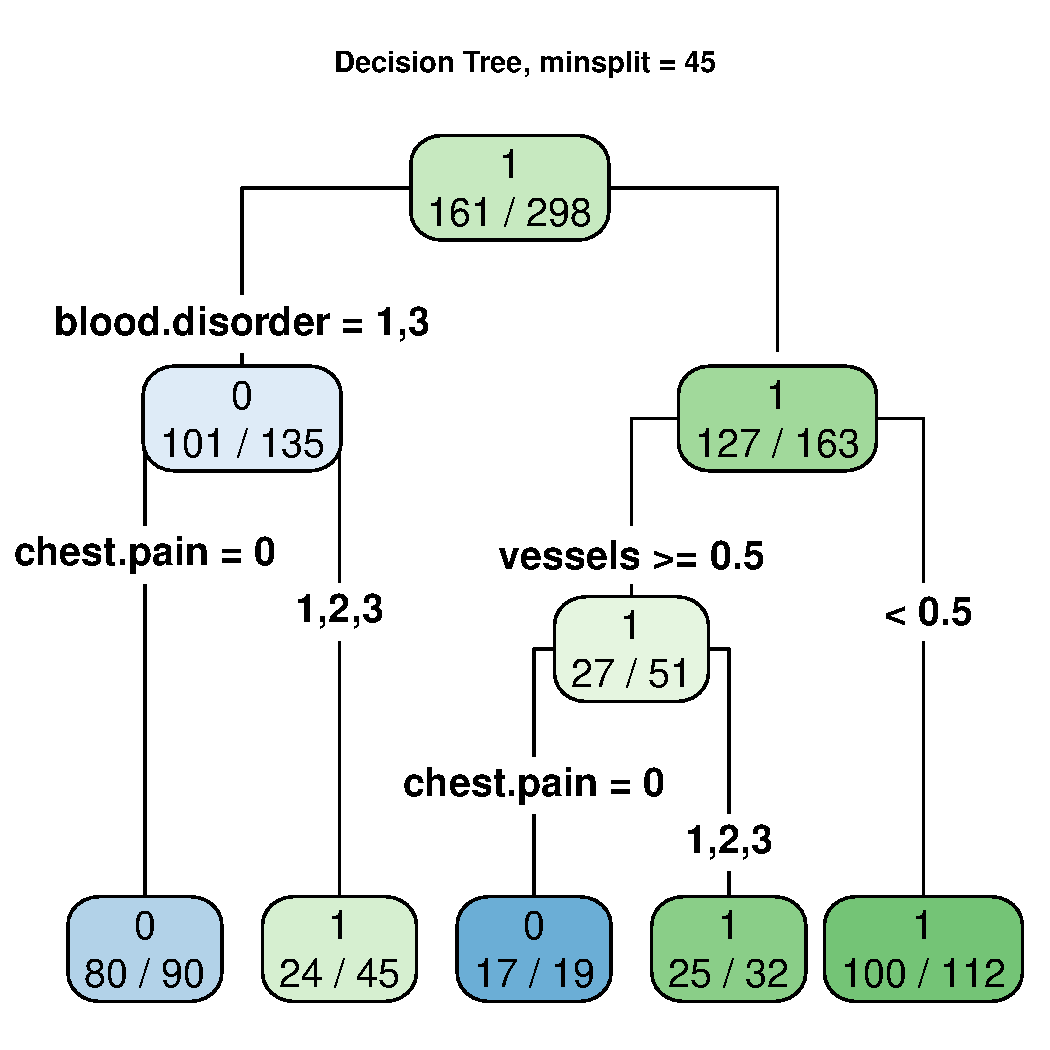
\includegraphics[width=0.45\linewidth]{32.DecisionTree-45.pdf}
    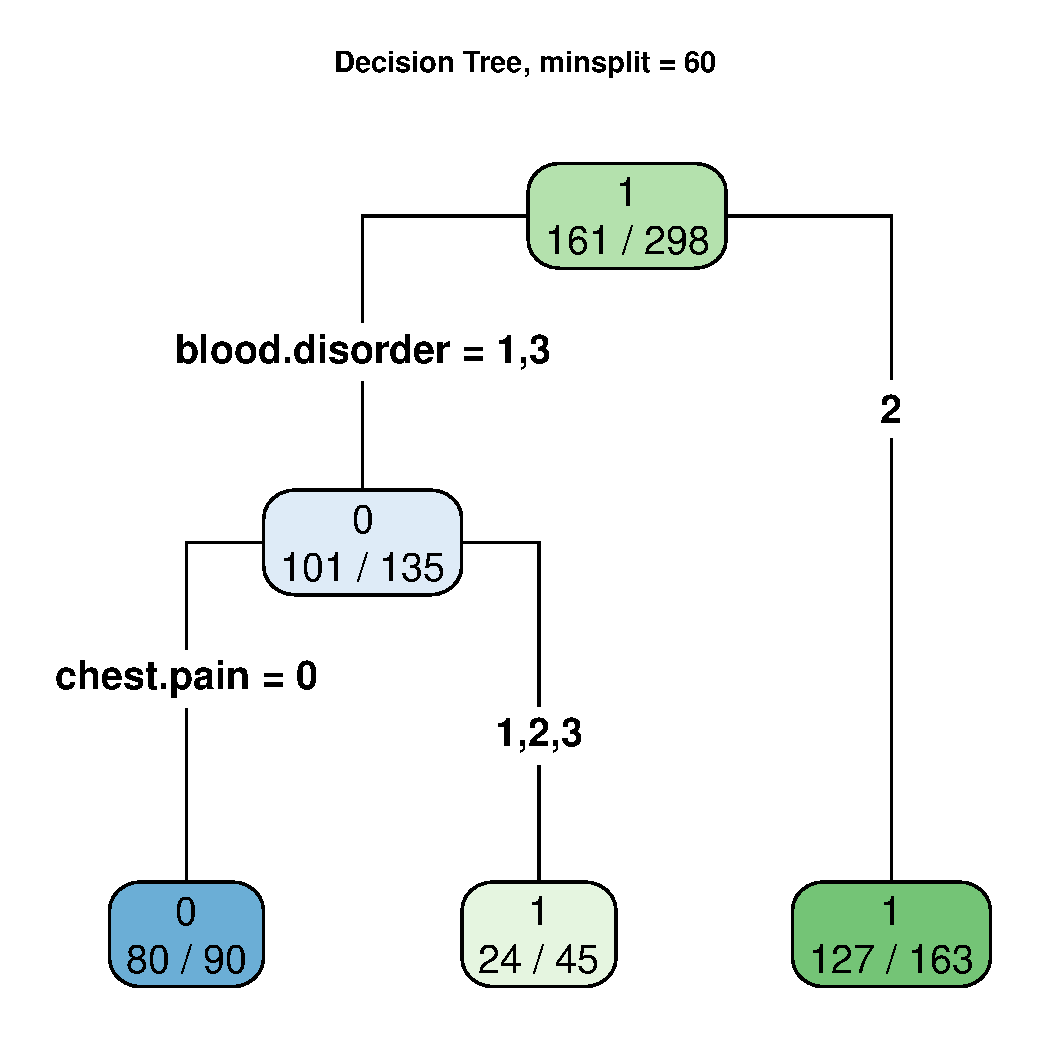
\includegraphics[width=0.45\linewidth]{32.DecisionTree-60.pdf}
    \caption{\centering Left: Moderate 45-minsplit decision tree; Right: Underfitting 60-minsplit decision tree}
\end{figure}

Choosing the 'best' model amongst all decision trees is rather a nuanced task due to the complex relationship between the \texttt{minsplit} hyperparameter with TPR-FPR metrics. For now, these two decision trees are left for further investigation:
\begin{itemize}
    \item \textbf{Information gain, \( \texttt{minsplit} = 30 \)}
    \item \textbf{Gini, \( \texttt{minsplit} = 45 \)}
\end{itemize}


\subsection{Logistic regression}


\subsubsection{Methodology}

Logistic regression is a regression model that estimates the \textit{log-odds} of an event as a linear combination of features:

\begin{align*}
    \ln \frac{\hat p}{1 - \hat p} = \hat\beta_0 + \hat\beta_1 X_1 + \cdots + \hat\beta_k X_k
\end{align*}

where \( \hat p \) is the estimator of \( \mathbb P[Y = 1] \), \( \hat\beta_0, \hat\beta_1, \cdots, \hat\beta_k \) are estimates of the linear coefficients. Unlike the usual linear regression, logistic regression has less assumption on its variable. For example, normality of independence variables is not required, hence it is not expected that logistic regression would better-fit on standardised data than the original one.

\begin{figure}[h]
    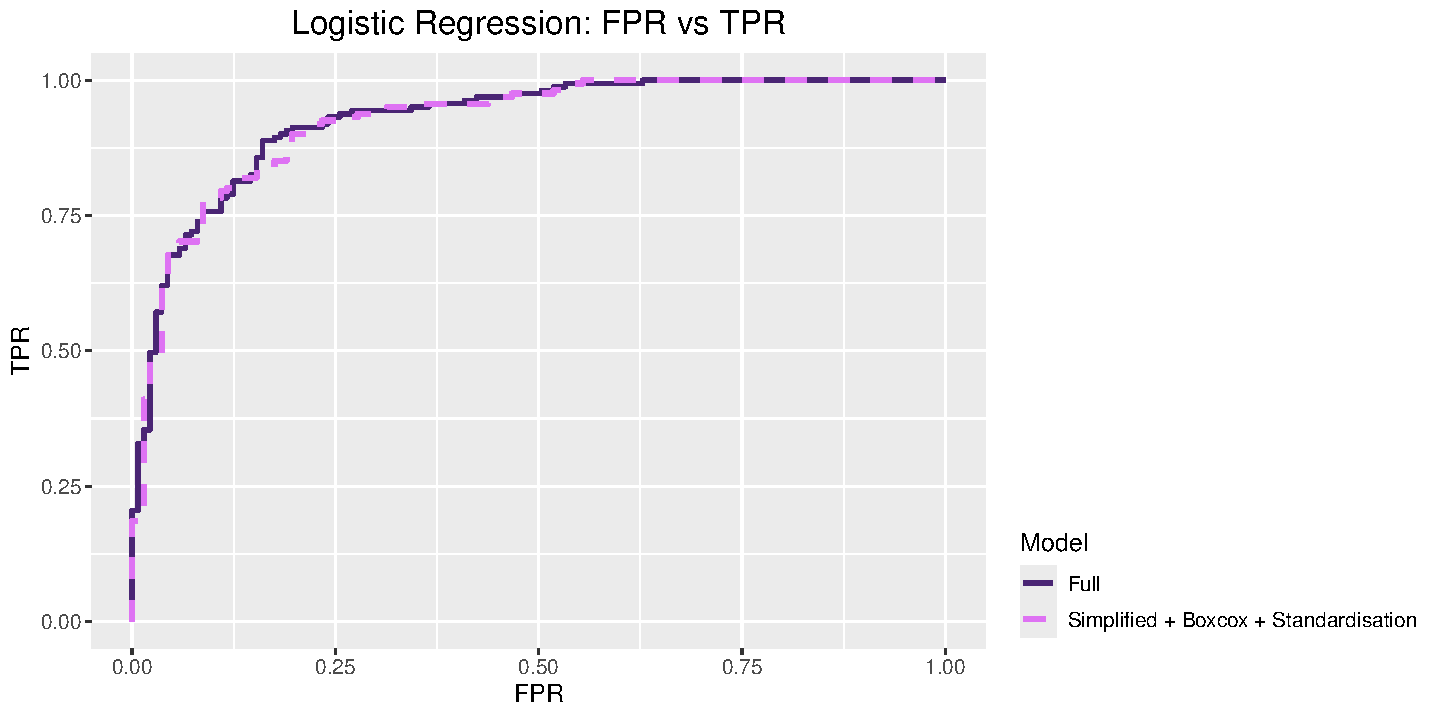
\includegraphics[width=\linewidth]{33.LogisticRegression.pdf}
    \caption{\centering ROC curve for logistic models}
\end{figure}

\subsubsection{Experiments \& Results}
Indeed, two logistic models are tested, a full model on all \( 12 \) features, and a simplified model on a Box-Cox, standardised version of only \( 9 \) significant features. They yields relatively similar results: investigation on the ROC curves produced by the two models shows that they pretty much overlap, except when \( \textrm{FPR} \approx 0.125 \) when the curve of the simplified model concaves down.

% \begin{table}[h]
%     \centering
%     \begin{tabular}{ccc}
%         \toprule
%         Logistic Regression
%             & \textbf{Full}
%             & \textbf{Box-Cox, Simplified\footnotemark{}}
%         \\
%         \midrule
%         \textbf{AUC}
%             & \( 0.9268 \)    
%             & \( 0.9235 \)
%         \\
%         \bottomrule
%     \end{tabular}
    
%     \raggedright
%     \( ^2 \) {\small \texttt{fbs}, \texttt{bp} and \texttt{chol} are excluded from the model}
    
%     \centering
%     \vspace{4pt}
%     \caption{}
% \end{table}

It can also be seen from the model coefficients that features contributing the most to the prediction of disease include \texttt{chest.pain}, \texttt{sex}, \texttt{blood.disorder} and \texttt{vessels}. There is a similarity between logistic models and decision trees, in the sense that these set of features stand as strong predictors for disease.

\begin{table}[h]
    \centering
    \begin{tabular}{lrr}
        \toprule
        \textbf{Feature} & \textbf{Estimate\footnotemark{}} & \textbf{p-value}\\
        \midrule
        \bf chest.pain3 & \bf 1.88 & \bf 0.0031\\
        \midrule
        \bf chest.pain2 & \bf 1.86 & \( \bf <  0.0001 \) \\
        \midrule
        \bf sex1 & \bf -1.31 & \bf 0.0085\\
        \midrule
        blood.disorder3 & -1.28 & 0.0954\\
        \midrule
        \bf chest.pain1 & \bf 1.11 & \bf 0.0437\\
        \midrule
        \bf vessels & \bf -0.80 & \( \bf < 0.0001 \)\\
        \midrule
        angina1 & -0.76 & 0.0716\\
        \midrule
        \bf st.depression & \bf -0.69 & \bf 0.0040\\
        \midrule
        rest.ecg1 & 0.65 & 0.0785\\
        \midrule
        \bf heart.rate & \bf 0.53 & \bf 0.0242\\
        \midrule
        (Intercept) & 0.44 & 0.6332\\
        \midrule
        rest.ecg2 & -0.30 & 0.8992\\
        \midrule
        \color{red}{chol} & 0.30 & 0.1504\\
        \midrule
        \color{red}{bp} & 0.29 & 0.1213\\
        \midrule
        blood.disorder2 & 0.21 & 0.7880\\
        \midrule
        \color{red}{fbs1} & 0.19 & 0.7367\\
        \midrule
        age & 0.01 & 0.9661\\
        \bottomrule
    \end{tabular}

    \raggedright
    \( ^\# \) {\small \textbf{bold values} indicate significant features (\( \alpha = 0.05 \))}
    
    \( ^3 \) {\small sorted by magnitude of coefficients}

    \centering
    \vspace{4pt}
    \caption{Description of the logistic model}
\end{table}



\section{Model validation and comparison}

As previous chapter selects the top candidate(s) from three family of models, this chapter describes the full validation of the models and report the most notable results from the process.

\begin{figure}[h]
    \centering
    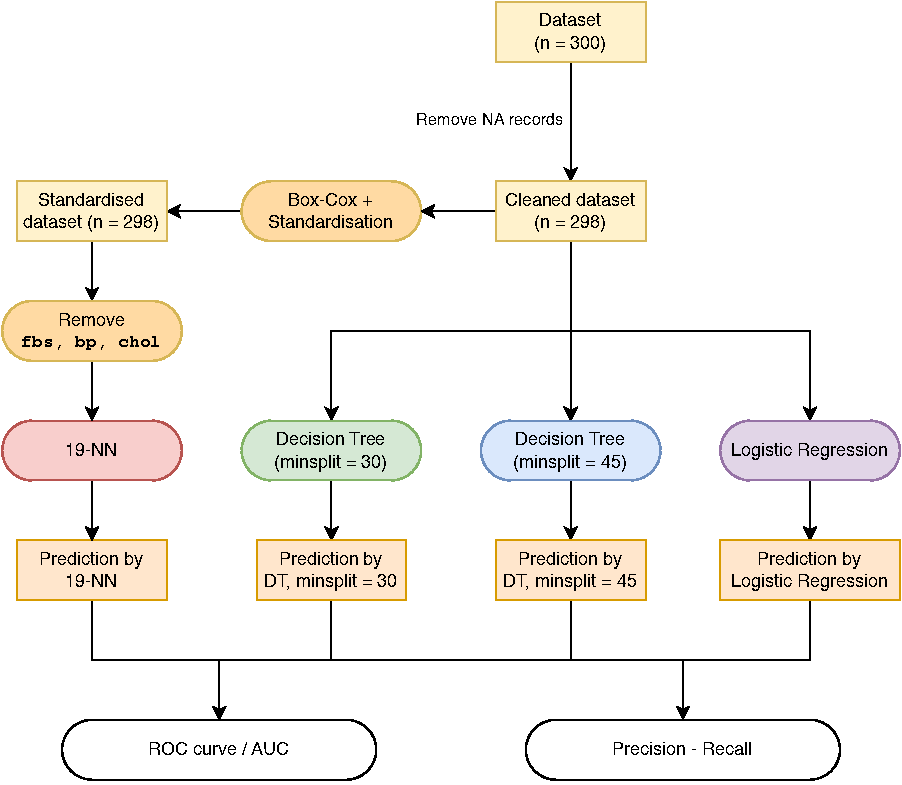
\includegraphics[width=\linewidth]{40.Validation-Diagram.pdf}
    
    \caption{\centering Process of models validation}
\end{figure}

The data pipeline starts with a full dataset of \( n = 300 \) records, two of which with unrecorded fields are then removed. A derivation of the dataset is generated by applying Box-Cox transformation and standardisation to all features, regarding categorical values as if they were numerical. The derived dataset is then fed to the \( 19 \)-NN model for training, whilst other models (logistic, decision trees) are given the cleaned, untransformed dataset. Each model produces a corresponding prediction result, which are then evaluated on the basis of (a) ROC-curve / AUC-score and (b) Precision — Recall curve.




\subsection{ROC - AUC (Receiver Operating Characteristic curve and Area Under the Curve)}

\begin{figure}[H]
    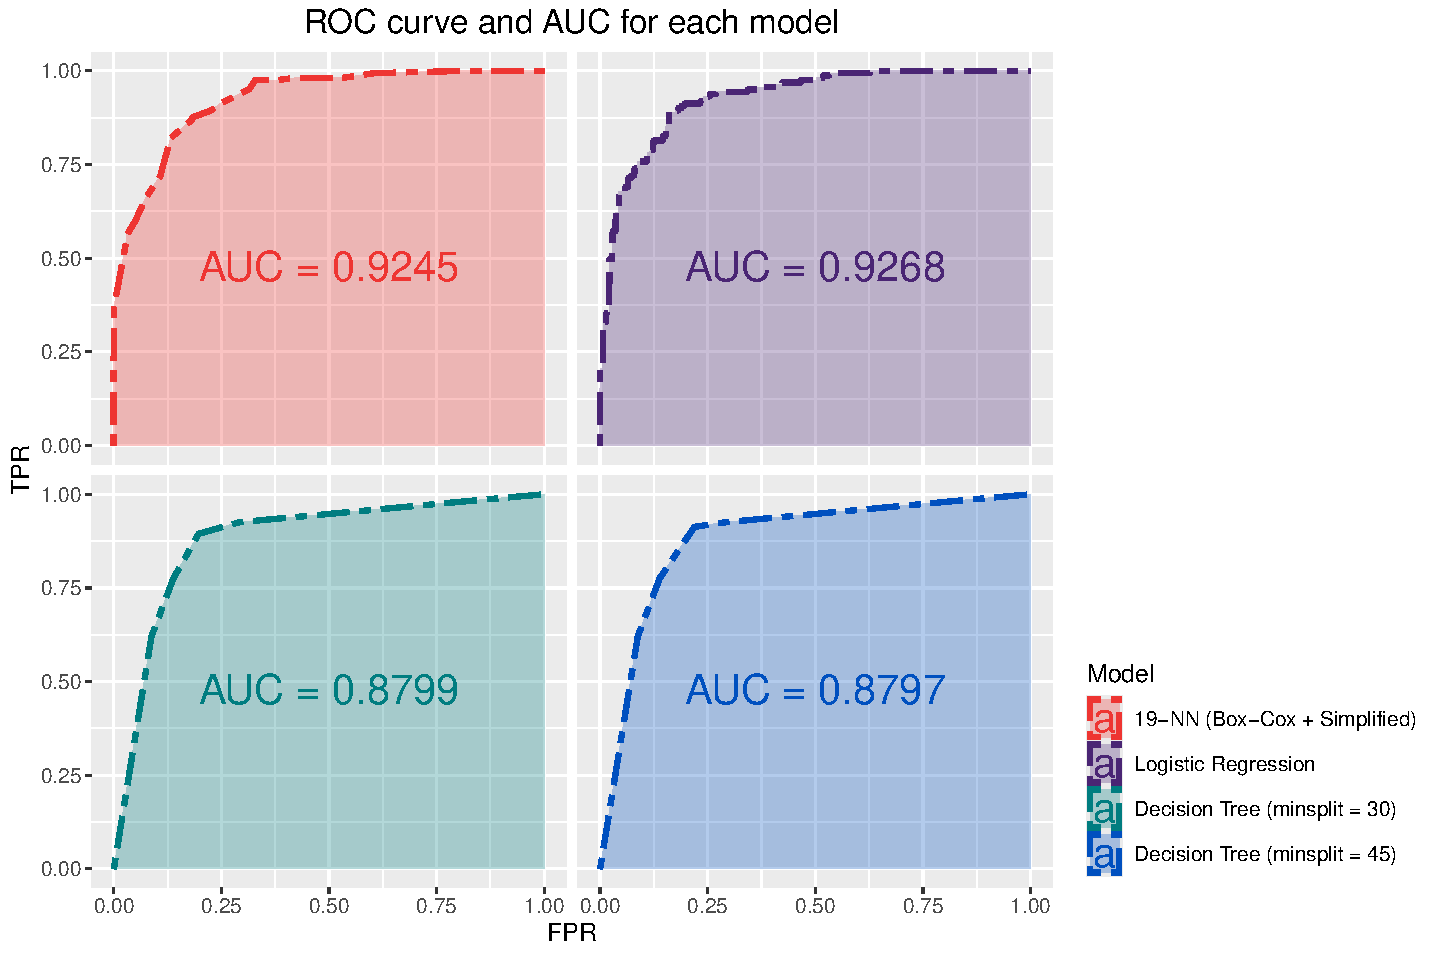
\includegraphics[width=\linewidth]{40.ROCs.pdf}
    \caption{\centering ROC curves and AUC for each model}
\end{figure}

Surprisingly, \( 19 \)-NN and logistic model produce similar ROC curves, despite having different modelling methodologies. It is less so for decision trees, as their alike curves can be explained by the analogous inner mechanisms of their structure.

In terms of AUC score, \( 19 \)-NN and logistic model give impressive scores of \( 0.9245 \) and \( 0.9268 \) respectively, whilst decision trees only yield less impressive scores from \( 0.8797 \) to \( 0.8799 \). The former models excel by considering exhaustive combinations of features, whilst the latter models suffer from overgeneralisation by only considering the most important features and skipping the details.





\subsection{Precision - Recall (TPR)}
\begin{figure}[H]
    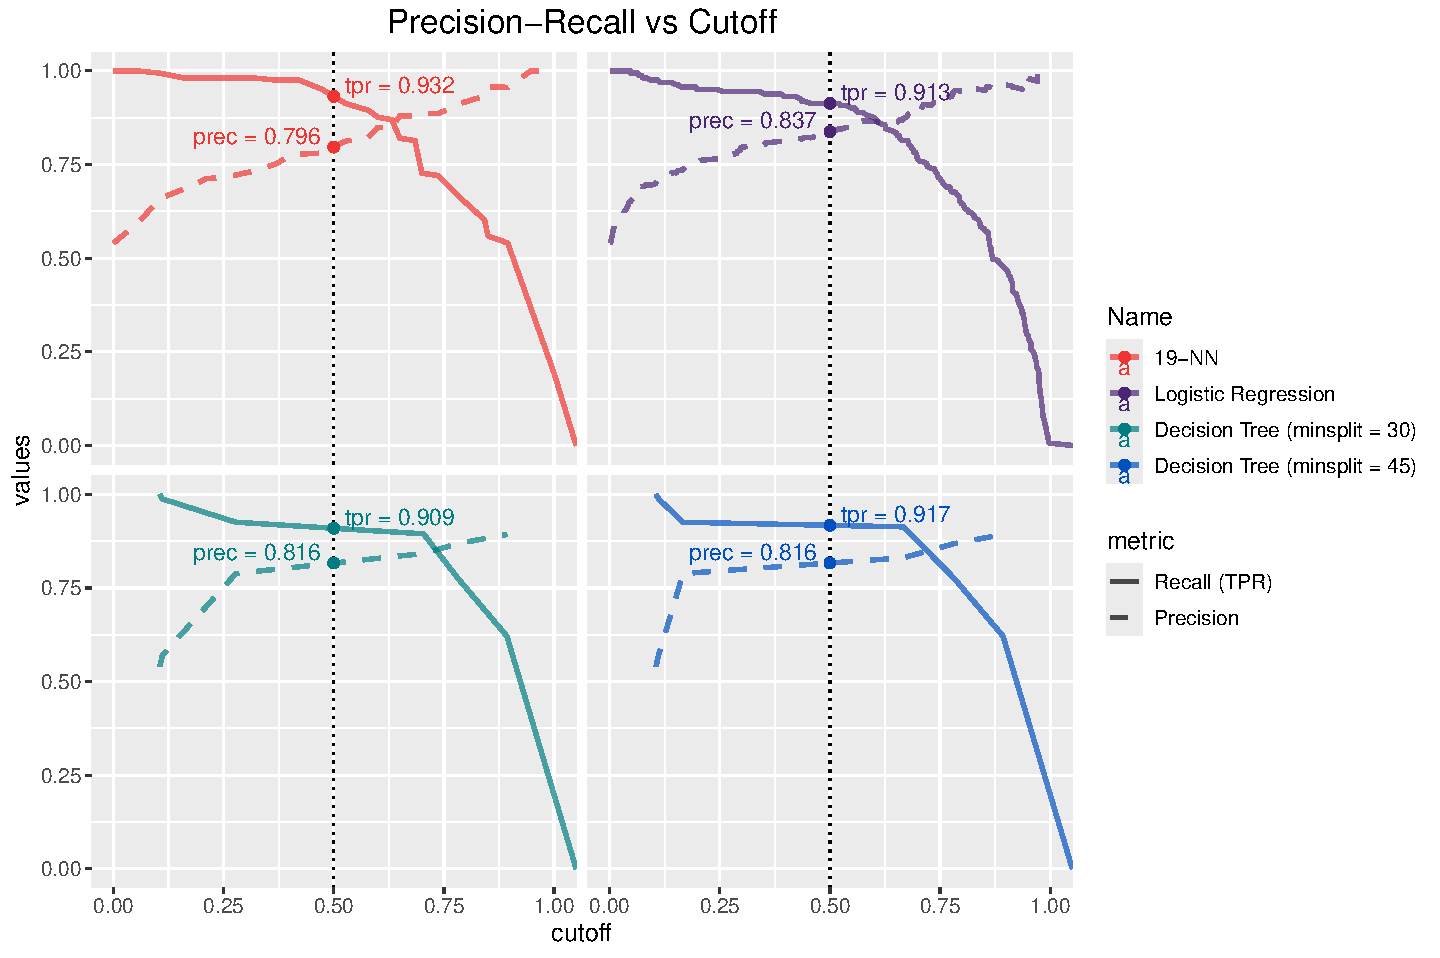
\includegraphics[width=\linewidth]{40.TPRs.pdf}
    \caption{\centering Percision/Recall -- Cutoff curves for each model}
\end{figure}

As the cutoff threshold increases, precision increases gradually whilst recall (TPR) decreases substantially, especially after the \( 0.5 \) threshold. Comparing models at the standard threshold of \( \delta = 0.5 \), it is observed that no models outperform the others in terms of precision and recall. \( 19 \)-NN tops at a \( 0.932 \) recall but fails at a low \( 0.796 \) precision, whilst logistic model observes a humble \( 0.913 \) recall but an impressive \( 0.837 \) precision. Decision trees are somewhat in between, with the \(45\)-minsplit model having a moderate \( 0.917 \) recall and \( 0.816 \) precision. 

\begin{figure}[h]
    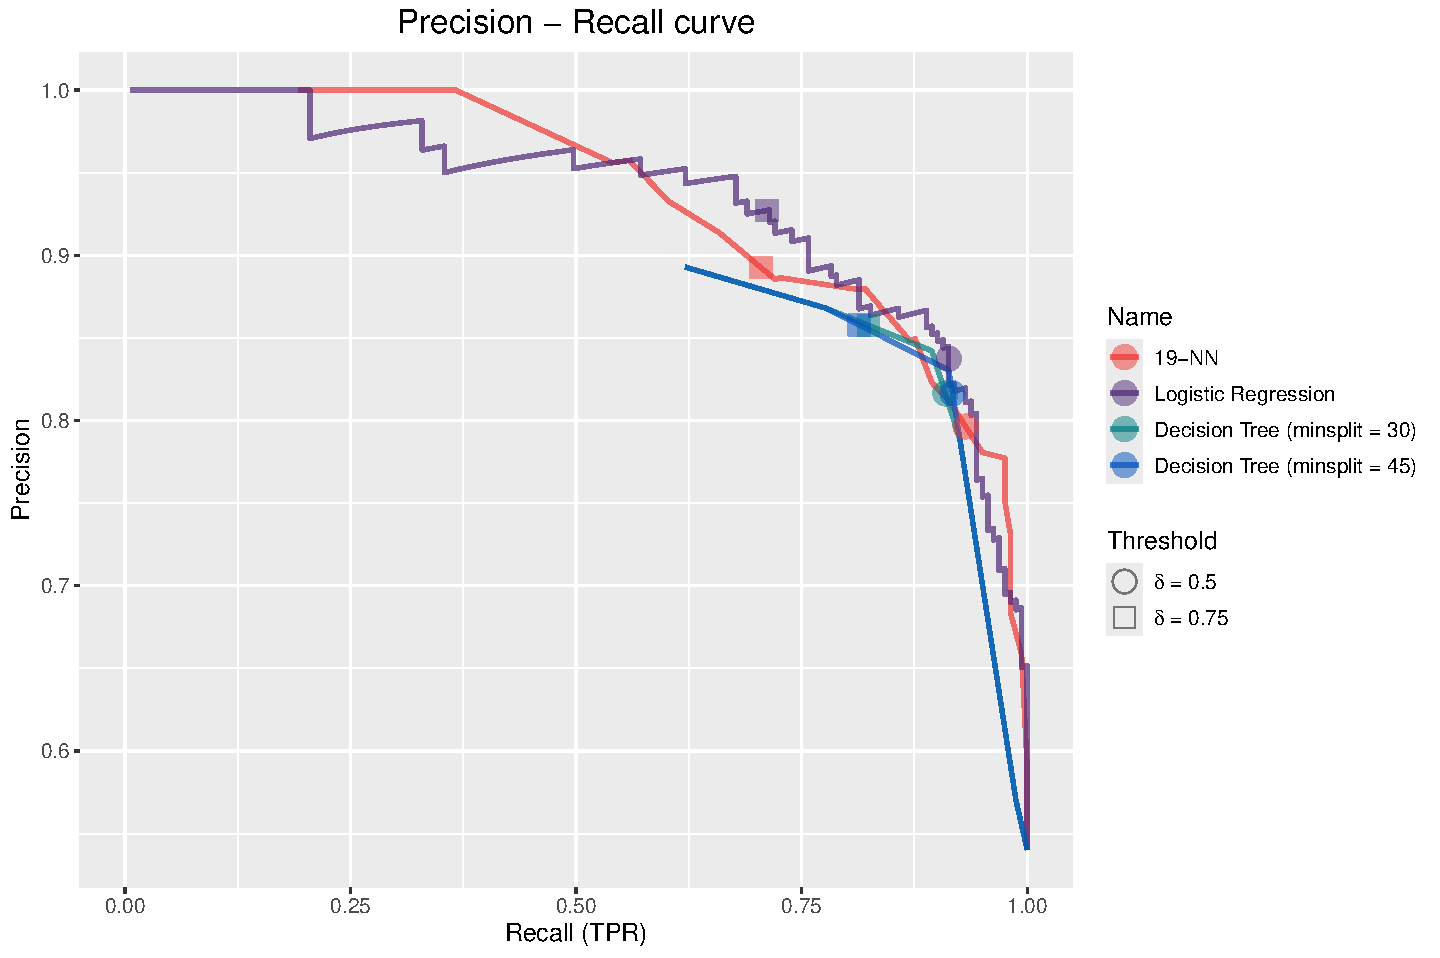
\includegraphics[width=\linewidth]{40.Precision-Recall.pdf}
    \caption{\centering Percision -- Recall curve}
\end{figure}

As the threshold is moved to \( \delta = 0.75 \), decision trees perform better in recall whilst logistic model and \( 19 \)-NN improve in precision. Concaveness around the \( \delta = 0.75 \) threshold is observed on the precision-recall curve of the \( 19 \)-NN model, whilst logistic model generally still performs well around this region.



\section{Conclusion and comments}

This report illustrates the comparisons between each type of models predicting heart disease based solely on specific demographical and clinical measures. In general, a \( k \)-nearest neighbour model, where \( k = 19 \), and logistic regression model outperform decision trees, with an AUC-score of around \( 0.93 \) compared to \( 0.88 \). Precision-recall-wise, logistic model shows performance stable lead around the \( \delta = 0.75 \) threshold, whilst \( 19 \)-NN lags behind.

For real-life application, \textbf{this report would support a logistic regression model}, thanks to its interpretibility and goodness-of-fit compared to other models. Indeed, this model illustrates solid performance in all metrics, with the highest AUC-score and a stable precision-recall curve. Also, by looking at the coefficients of the model, one can deduce the importance of each feature in contributing to the disease status.

This is not present in other experiments. Decision trees, despite its simplicity, fail to give reliable results and a detailed explaination, as factors like \texttt{heart.rate} or \texttt{angina} are never considered. In contrast, although the best nearest neighbour model perform equivalently to a logistic model, there is no simple explaination on how the model would interpret the features other than a simple distance-based rule. Another drawback of \(k\)-NN is \textit{the curse of dimensionality}, as the model is essentially working on a \( \mathbb R^9 \) numerical space in which the difference in distances are negligible. Had the dataset got more features, this effect would have been a significant problem.

For further analysis, this report would suggest that some kind of dimensionality reduction is applied on the data (for instance, Principal Component Analysis, \( \mathbb R^9 \mapsto \mathbb R^2 \)) so that nearest neighbour models can work on a less-dimensional, compact space. Other models such as Na\"ive Bayes can be considered for similar small datasets. Finally, one of the big challenges in this report is the size of the dataset, with only \( n = 298 \) records after cleaning. One could try evaluting the models on a \( 918 \)-record dataset from the UCI Machine Learning Repository \citep{extradataset} and would probably produce more reliable results.

\nocite{*}
\setlength{\bibsep}{10pt}
\bibliography{bbtex.bib}  

% bib file to produce the bibliography                                                  

\end{document}
